\documentclass[11pt,a4paper]{report}

% Packages
% Packages
\usepackage[utf8]{inputenc}
\usepackage{graphicx}
\usepackage{amsmath}
\usepackage{amsfonts}
\usepackage{amssymb}
\usepackage{cite} % For IEEE-style citations
\usepackage[spanish]{babel} % Language support for Spanish
\usepackage{hyperref} % For hyperlinks
\usepackage{geometry} % For setting margins
\usepackage{titlesec} % For title formatting
\usepackage{fancyhdr} % For header and footer
\usepackage{helvet} % For Arial font
\usepackage{ragged2e} % For justified text
\usepackage{setspace} % For line spacing control
\usepackage{float} % For figure and table placement
\usepackage{caption} % For customizing captions
\usepackage[titles]{tocloft} % For customizing Table of Contents
\usepackage{appendix} % For managing appendices
\usepackage{etoolbox} % For advanced LaTeX commands
\usepackage{lipsum}
\renewcommand{\familydefault}{\sfdefault} % Set font to Arial

% Page Layout
\geometry{left=3cm, right=2.5cm, top=3cm, bottom=2.5cm}

\setlength{\parindent}{0pt} % No indentation for paragraphs
\setstretch{1.5} % Line spacing

% Custom command to enforce no indentation
\newcommand{\noindentation}{\setlength{\parindent}{0pt} \raggedright}

% *** Custom chapter title format with 14pt font size ***
\titleformat{\chapter}[block]
  {\normalfont\fontsize{14pt}{14pt}\selectfont\bfseries}
  {\thechapter\ }{0pt}{\fontsize{14pt}{16pt}\selectfont\bfseries}

% *** Adjust spacing after chapter titles ***
\titlespacing*{\chapter}{0pt}{-20pt}{5pt} % Left indent: 0pt, Space before: -20pt (default adjustment), Space after: 5pt


% Custom title format for RESUMEN and ABSTRACT
\titleformat{name=\chapter,numberless}[block]
  {\centering\normalfont\fontsize{14pt}{16pt}\selectfont\bfseries}
  {}{0pt}{\vspace{8pt}}

  
% *** Custom section title format with 14pt font size ***
\titleformat{\section}
  {\normalfont\fontsize{14pt}{14pt}\selectfont\bfseries}{\thesection\ \ }{0pt}{\fontsize{14pt}{14pt}\selectfont\bfseries}

% *** Adjust spacing after section titles and set left indentation ***
\titlespacing*{\section}{1.25cm}{*}{8pt} % Left indent: 1.25cm, Space before: default (*), Space after: 8pt

% *** Custom subsection title format (Unnumbered and Starts on New Line) ***
\titleformat{\subsection}[block] % "block" style ensures content starts on a new line
{\normalfont\fontsize{12pt}{14pt}\selectfont\bfseries}{}{0pt}{\fontsize{12pt}{14pt}\selectfont\bfseries}


% *** Adjust spacing after unnumbered subsection titles and set left indentation ***
\titlespacing*{\subsection}{1.25cm}{*}{8pt} % Left indent: 1.25cm, Space before: default (*), Space after: 8pt




% Header and Footer
\fancypagestyle{plain}{
  \fancyhf{}
  %\fancyhead[L]{\textit{Escuela Politécnica Nacional}}
  \fancyfoot[C]{\thepage}
  \renewcommand{\headrulewidth}{0pt}
}

\addto\captionsspanish{
  \renewcommand{\contentsname}{\centering ÍNDICE DE CONTENIDO}
}


\captionsetup[figure]{
    labelsep=period,
    labelfont={bf},
    textfont=small,
    name=Figura,
}

\captionsetup[table]{
    labelsep=period,
    labelfont={bf},
    textfont=small,
    name=Tabla,
}
% Custom Table of Contents formatting
\renewcommand{\cftchapfont}{\normalfont\normalsize} % Chapter entries in ToC
\renewcommand{\cftsecfont}{\normalfont\normalsize}  % Section entries in ToC
\renewcommand{\cftsubsecfont}{\normalfont\normalsize} % Subsection entries in ToC

\renewcommand{\cftchappagefont}{\normalfont\normalsize} % Chapter page numbers in ToC
\renewcommand{\cftsecpagefont}{\normalfont\normalsize}  % Section page numbers in ToC
\renewcommand{\cftsubsecpagefont}{\normalfont\normalsize} % Subsection page numbers in ToC

% Set uniform line spacing in ToC
\begingroup
\renewcommand{\cftbeforetoctitleskip}{0pt}
\renewcommand{\cftaftertoctitleskip}{0pt}
\setstretch{1.5} % Ensure 1.5 line spacing in ToC
\makeatletter
\patchcmd{\tableofcontents}{\@starttoc}{\begingroup\setstretch{1.5}\@starttoc}{}{}
\makeatother
\endgroup



%%%%%%%%%%%%%%%%%%%%%%%%%%%%%%%%%%%%%%%%%%%%%%%%%%%%%%%%%%%%%%%%%%%%%%%%%%%%%%%%%%%%%%%%%%%%%%%%%%%%%%%%%%%%%%%%%%%%%%%%%%%%
\begin{document}

% Set page numbering to Roman numerals
\pagenumbering{roman}

% Include sections
\begin{titlepage}
    \centering
    \vspace{1cm}
    {\fontsize{24pt}{24pt}\selectfont \bfseries ESCUELA POLITECNICA NACIONAL \par}
    
    \vspace{1.5cm}
    {\fontsize{16pt}{16pt}\selectfont \bfseries FACULTAD DE INGENIERIA ELECTRICA Y  ELECTRONICA \par}
    \vspace{2cm}
        {\fontsize{14pt}{14pt}\selectfont \bfseries NOMBRE DEL PROYECTO EN EL QUE SE DESARROLLA EL TRABAJO DE INTEGRACIÓN CURRICULAR \par}
    \vspace{2cm}
     {\fontsize{14pt}{14pt}\selectfont \bfseries NOMBRE DEL COMPONENTE \par}
    \vspace{2cm}



    {\fontsize{12pt}{12pt}\selectfont \bfseries TRABAJO DE INTEGRACIÓN CURRICULAR PRESENTADO COMO REQUISITO PARA LA OBTENCIÓN DEL TÍTULO DE INGENIERO EN ELECTRÓNICA Y AUTOMATIZACIÓN \par}
         
    \vspace{2cm}
    
     {\fontsize{12pt}{12pt}\selectfont \bfseries Nombre Del Estudiante \par}
    \vspace{0.1cm}
    
     {\fontsize{12pt}{12pt}\selectfont \bfseries email@epn.edu.ec \par}
    \vspace{0.1cm}

        {\fontsize{12pt}{12pt}\selectfont \bfseries Director: Ing. William Chamorro, PhD. \par}
    \vspace{0.1cm}
    
     {\fontsize{12pt}{12pt}\selectfont \bfseries william.chamorro@epn.edu.ec \par}
    \vspace{0.1cm}

    
    \vspace{2cm}
    {\fontsize{12pt}{12pt}\selectfont \bfseries DMQ, julio 2024 \par}
 
\end{titlepage}

\chapter*{CERTIFICACIONES}
\addcontentsline{toc}{chapter}{CERTIFICACIONES} 

\justifying
Yo, NOMBRE DEL ESTUDIANTE declaro que el trabajo de integración curricular aquí descrito es de mi autoría; que no ha sido previamente presentado para ningún grado o calificación profesional; y, que he consultado las referencias bibliográficas que se incluyen en este documento.

\vspace{2cm}

\begin{center}
    \rule{8cm}{0.5pt}\\ % Horizontal line
    \textbf{Nombre del estudiante} % Name
\end{center}

\vspace{2cm}
\justifying
Certifico que el presente trabajo de integración curricular fue desarrollado por \textbf{NOMBRE DEL ESTUDIANTE}, bajo mi supervisión.

\vspace{2cm}

\begin{center}
    \rule{8cm}{0.5pt}\\ % Horizontal line
    \textbf{Ing. William Chamorro, PhD.} % Name
\end{center}




\chapter*{DECLARACIÓN DE AUTORÍA}
\addcontentsline{toc}{chapter}{DECLARACIÓN DE AUTORÍA} 

\justifying
A través de la presente declaración, afirmamos que el trabajo de integración curricular aquí descrito, así como el (los) producto(s) resultante(s) del mismo, son públicos y estarán a disposición de la comunidad a través del repositorio institucional de la Escuela Politécnica Nacional; sin embargo, la titularidad de los derechos patrimoniales nos corresponde a los autores que hemos contribuido en el desarrollo del presente trabajo; observando para el efecto las disposiciones establecidas por el órgano competente en propiedad intelectual, la normativa interna y demás normas.

\vspace{2cm}

\raggedright
    \textbf{NOMBRE DEL ESTUDIANTE} % Name
    \vspace{0.1cm}
    
    \textbf{WILLIAM OSWALDO CHAMORRO HERNÁNDEZ, PHD.} % Name


    
\chapter*{} % Empty chapter to manage spacing
\vspace*{-2cm} % Adjust the vertical position of the title
\begin{center}
    \textbf{\Large DEDICATORIA} % Center and increase the size of the title
\end{center}
\justifying
Dedico este trabajo a todas las personas que han sido parte fundamental en mi vida y en este proyecto. A mi familia, por su apoyo incondicional y amor constante, y a mis amigos, cuya compañía y ánimo han hecho este viaje más agradable y valioso.

\chapter*{AGRADECIMIENTO}
\addcontentsline{toc}{chapter}{AGRADECIMIENTO} 

\justifying
Quiero expresar mi más sincero agradecimiento a todas las personas que han sido fundamentales para la realización de este trabajo de integración curricular y para mi desarrollo a lo largo de toda la carrera.
\newpage

\tableofcontents
\chapter*{RESUMEN}
\addcontentsline{toc}{chapter}{RESUMEN} % Adds RESUMEN to the Table of Contents
\justifying
(Máximo 250 palabras)
En el presente trabajo de integración curricular se plantea como fin el control de un brazo robótico de 5 grados de libertad para tareas de paletización. El brazo que se utilizará fue ensamblado en el TIC “Ensamblaje y Control de un Robot con Arquitectura Antropomórfica de cinco grados de libertad”, en este TIC se realizó el control tanto en alto nivel como en bajo nivel. Tomando como base dichos controladores se realizó la adaptación necesaria para que el robot realice tareas de paletización. Además, se desarrolló una interfaz gráfica en MATLAB-Simulink donde se encuentra implementada la cinemática para el control del movimiento angular de cada uno de los motores, en dicha interfaz gráfica el usuario debe ingresar las coordenadas de inicio y fin para realizar las tareas de paletización. Adicionalmente para complementar al robot ensamblado se manufacturó un efector final tipo pinza de 2 dedos cuyos planos de diseño se obtuvieron del proyecto de investigación PIMI-14-04. Al culminar con este proyecto, el laboratorio de Sistemas de control del DACI contará con un prototipo de un brazo robótico de 5 GDL que tenga la capacidad de realizar tareas de paletización para realizar prácticas de laboratorio de la asignatura de Robótica. Estos resultados consolidados representarán no solo la culminación exitosa de los esfuerzos invertidos en el proyecto, sino también una contribución significativa para fortalecer las capacidades del laboratorio y facilitar la realización de prácticas educativas aplicadas en el entorno de la robótica.

\vspace{1cm}
\noindent \textbf{PALABRAS CLAVE:} antropomórfico, paletización, grados de libertad.

\newpage

 
\chapter*{\centering ABSTRACT}
\addcontentsline{toc}{chapter}{ABSTRACT} % Adds RESUMEN to the Table of Contents


\justifying
(Máximo 250 palabras)
This curricular integration project aims to control a 5-degree-of-freedom robotic arm for palletizing tasks. The arm to be used was assembled in the TIC project "Assembly and Control of a Robot with an Anthropomorphic Architecture of Five Degrees of Freedom," in which both high-level and low-level control were implemented. Based on these controllers, the necessary adaptation was made for the robot to perform palletizing tasks. Additionally, a graphical interface in MATLAB-Simulink was developed, where the kinematics for controlling the angular movement of each motor is implemented. In this graphical interface, the user must enter the start and end coordinates to carry out the palletizing tasks. Furthermore, to complement the assembled robot, a two-finger gripper-type end effector was manufactured, with design plans obtained from the research project PIMI-14-04. Upon completion of this project, the Control Systems Laboratory of DACI will have a prototype of a 5-DOF robotic arm capable of performing palletizing tasks for laboratory practices in the Robotics course. These consolidated results will not only represent the successful culmination of the efforts invested in the project but also a significant contribution to strengthening the laboratory's capabilities and facilitating the execution of applied educational practices in the field of robotics.

\vspace{1cm}
\noindent \textbf{KEYWORDS:} anthropomorphic, palletizing, degrees of freedom.

\newpage

% Chapters

% Start Arabic page numbering from Chapter 1
\clearpage
\pagenumbering{arabic}
\chapter{INTRODUCCIÓN}
\lipsum[1-3]\cite{herrera2015sliding}.

\section{Objetivo General}
\lipsum[1-3]\cite{herrera2015sliding}.
Realizar el control de un Robot con Arquitectura Antropomórfica de cinco grados de libertad que realice tareas de paletización \cite{chamorro2020high}.

\begin{figure}[H]
    \centering
    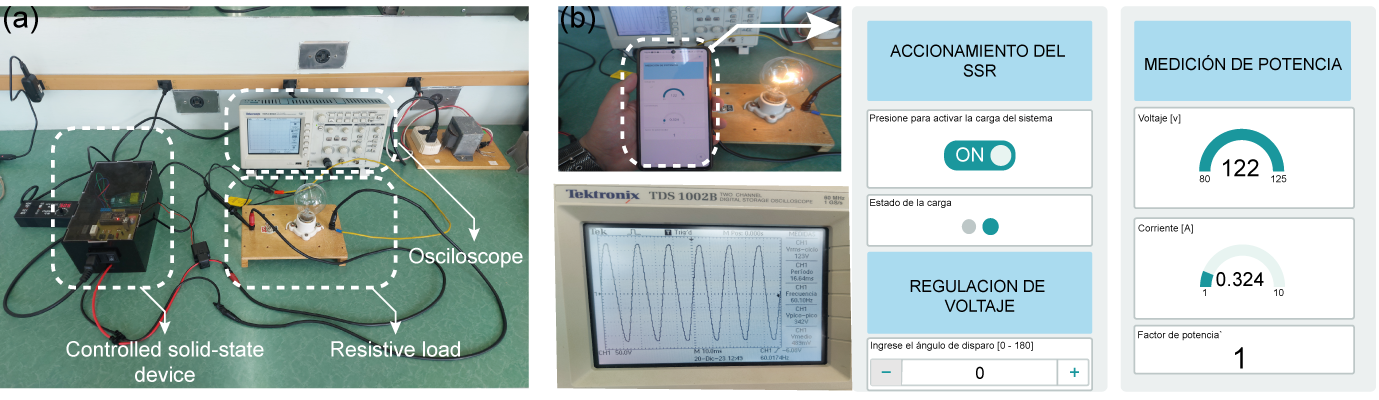
\includegraphics[width=\textwidth]{figuras/testR.png} % Replace with your image file path
    \caption{Gemelo Digital y Gemelo Físico.}
    \label{fig:gemelo_digital}
\end{figure}



\section{Objetivos Específicos}
\begin{itemize}
    \item Realizar revisión bibliográfica del TIC “Ensamblaje y Control de un Robot con Arquitectura Antropomórfica de cinco grados de libertad”.
    \item Adaptar el software de control en alto y bajo nivel para realizar tareas de paletización.
\end{itemize}

\section{Alcance}
Realizar una revisión bibliográfica del diseño del robot antropomórfico de cinco grados de libertad.

\section{Marco Teórico}
Realizar una revisión bibliográfica del diseño del robot antropomórfico de cinco grados de libertad
\subsection{Estado del Arte}

\lipsum[1-3]\cite{herrera2015sliding}.
\chapter{METODOLOGÍA}
% Include content for Chapter 2 here.
% For example:
\section{Tema 1}
Contenido de la sección sobre el efector final.

\begin{table}[H]
    \centering
    \caption{Datos Ejemplo en la Tabla.}
    \begin{tabular}{|c|c|c|}
        \hline
        Columna 1 & Columna 2 & Columna 3 \\ \hline
        Dato 1    & Dato 2    & Dato 3    \\ \hline
        Dato 4    & Dato 5    & Dato 6    \\ \hline
        Dato 7    & Dato 8    & Dato 9    \\ \hline
    \end{tabular}
    
    \label{tab:ejemplo}
\end{table}

\section{Tema 2}
Contenido sobre la incorporación del motor.

\chapter{RESULTADOS}
% Include content for Chapter 2 here.
% For example:
\section{Tema 1}
Contenido de la sección sobre el efector final.
\chapter{CONCLUSIONES Y RECOMENDACIONES}
% Include content for Chapter 2 here.
% For example:
\section{Conclusiones}
\lipsum[1-3]

\section{Recomendaciones}
\lipsum[1-3]

% *** Start of Appendix Configuration ***
\appendix % Start the appendix section

% Redefine the chapter command for appendices
\titleformat{\chapter}[block]
  {\normalfont\fontsize{14pt}{14pt}\selectfont\bfseries}
  {ANEXO \thechapter\ }{0pt}{\fontsize{14pt}{16pt}\selectfont\bfseries\vspace{1em}}

\renewcommand{\thechapter}{\Roman{chapter}} % Use Roman numerals for appendix chapters

% Adjust section numbering in the appendices
\renewcommand{\thesection}{\thechapter.\arabic{section}} % Section numbering as I.1, II.1, etc.
\renewcommand{\thesubsection}{\thesection.\arabic{subsection}} % Subsection numbering as I.1.1, II.1.1, etc.

% **Appendix Title ANEXO I**
\chapter{Título del Anexo I}

% **Section within Appendix I (e.g., I.1)**
\section{Sección del Anexo I}
Contenido de la sección 1 en el Anexo I.

% **Subsection within Appendix I (e.g., I.1.1)**
\subsection{Subsección del Anexo I}
Contenido de la subsección 1 en el Anexo I.


\chapter{Título anoexo2}
\section{Sección anexo 2}

% References
\renewcommand{\bibname}{REFERENCIAS BIBLIOGRÁFICAS}
\bibliographystyle{IEEEtran}
\bibliography{references}

\end{document}
